\documentclass[tikz,border=8pt]{standalone}
\usepackage[T1]{fontenc}
\usepackage{amsmath,amssymb}
\usepackage{xcolor}
\usepackage{tikz}
% Shared TikZ style for the DEV architecture diagrams.
% Requires only TikZ and standard TikZ libraries.
\usetikzlibrary{arrows.meta,backgrounds,calc,fit,positioning}

\definecolor{DevInk}{HTML}{172033}
\definecolor{DevMuted}{HTML}{526078}
\definecolor{DevLine}{HTML}{475569}
\definecolor{DevPanel}{HTML}{F8FAFC}
\definecolor{DevPanelBorder}{HTML}{CBD5E1}
\definecolor{DevContent}{HTML}{DBEAFE}
\definecolor{DevContentBorder}{HTML}{2563EB}
\definecolor{DevStyle}{HTML}{F3E8FF}
\definecolor{DevStyleBorder}{HTML}{9333EA}
\definecolor{DevStable}{HTML}{DCFCE7}
\definecolor{DevStableBorder}{HTML}{16A34A}
\definecolor{DevAllograph}{HTML}{FFEDD5}
\definecolor{DevAllographBorder}{HTML}{EA580C}
\definecolor{DevCritic}{HTML}{FEE2E2}
\definecolor{DevCriticBorder}{HTML}{DC2626}
\definecolor{DevLoss}{HTML}{FEF3C7}
\definecolor{DevLossBorder}{HTML}{D97706}

\tikzset{
  devtext/.style={font=\sffamily\small, text=DevInk, align=center},
  devbox/.style={
    devtext,
    draw=DevPanelBorder,
    fill=white,
    rounded corners=2.2mm,
    line width=0.75pt,
    inner xsep=3.2mm,
    inner ysep=2.4mm,
    minimum height=9mm
  },
  devinput/.style={devbox, draw=DevContentBorder, fill=DevContent},
  devcontent/.style={devbox, draw=DevContentBorder, fill=DevContent},
  devstyle/.style={devbox, draw=DevStyleBorder, fill=DevStyle},
  devstable/.style={devbox, draw=DevStableBorder, fill=DevStable},
  devallograph/.style={devbox, draw=DevAllographBorder, fill=DevAllograph},
  devcritic/.style={devbox, draw=DevCriticBorder, fill=DevCritic},
  devloss/.style={devbox, draw=DevLossBorder, fill=DevLoss},
  devgroup/.style={
    draw=DevPanelBorder,
    fill=DevPanel,
    rounded corners=3mm,
    line width=0.75pt,
    inner sep=4mm
  },
  devflow/.style={
    -{Latex[length=2.8mm,width=1.9mm]},
    draw=DevLine,
    line width=0.85pt,
    rounded corners=1.4mm
  },
  devaux/.style={
    devflow,
    draw=DevStableBorder,
    densely dashed
  },
  devlossflow/.style={
    devflow,
    draw=DevLossBorder,
    densely dashed
  },
  devlabel/.style={
    font=\sffamily\scriptsize,
    text=DevMuted,
    fill=white,
    inner sep=1.2pt
  },
  devgrouptitle/.style={
    font=\sffamily\bfseries\small,
    text=DevInk,
    fill=DevPanel,
    inner xsep=2mm,
    inner ysep=0.6mm
  },
  devnote/.style={
    font=\sffamily\scriptsize,
    text=DevMuted,
    align=left
  }
}



\tikzset{
  wholebox/.style={devbox, font=\sffamily\scriptsize, inner xsep=2.4mm,
    inner ysep=1.8mm, minimum height=8mm},
  wholeinput/.style={wholebox, draw=DevContentBorder, fill=DevContent},
  wholestyle/.style={wholebox, draw=DevStyleBorder, fill=DevStyle},
  wholestable/.style={wholebox, draw=DevStableBorder, fill=DevStable},
  wholeallograph/.style={wholebox, draw=DevAllographBorder, fill=DevAllograph},
  wholecritic/.style={wholebox, draw=DevCriticBorder, fill=DevCritic},
  wholeloss/.style={wholebox, draw=DevLossBorder, fill=DevLoss},
  styleflow/.style={devflow, draw=DevStyleBorder},
  criticflow/.style={devflow, draw=DevCriticBorder},
  thinbus/.style={draw=DevLine, line width=0.8pt, rounded corners=1.2mm},
  lossbus/.style={draw=DevLossBorder, line width=0.8pt, densely dashed,
    rounded corners=1.2mm},
  paneltitle/.style={devgrouptitle, font=\sffamily\bfseries\small}
}

\begin{document}
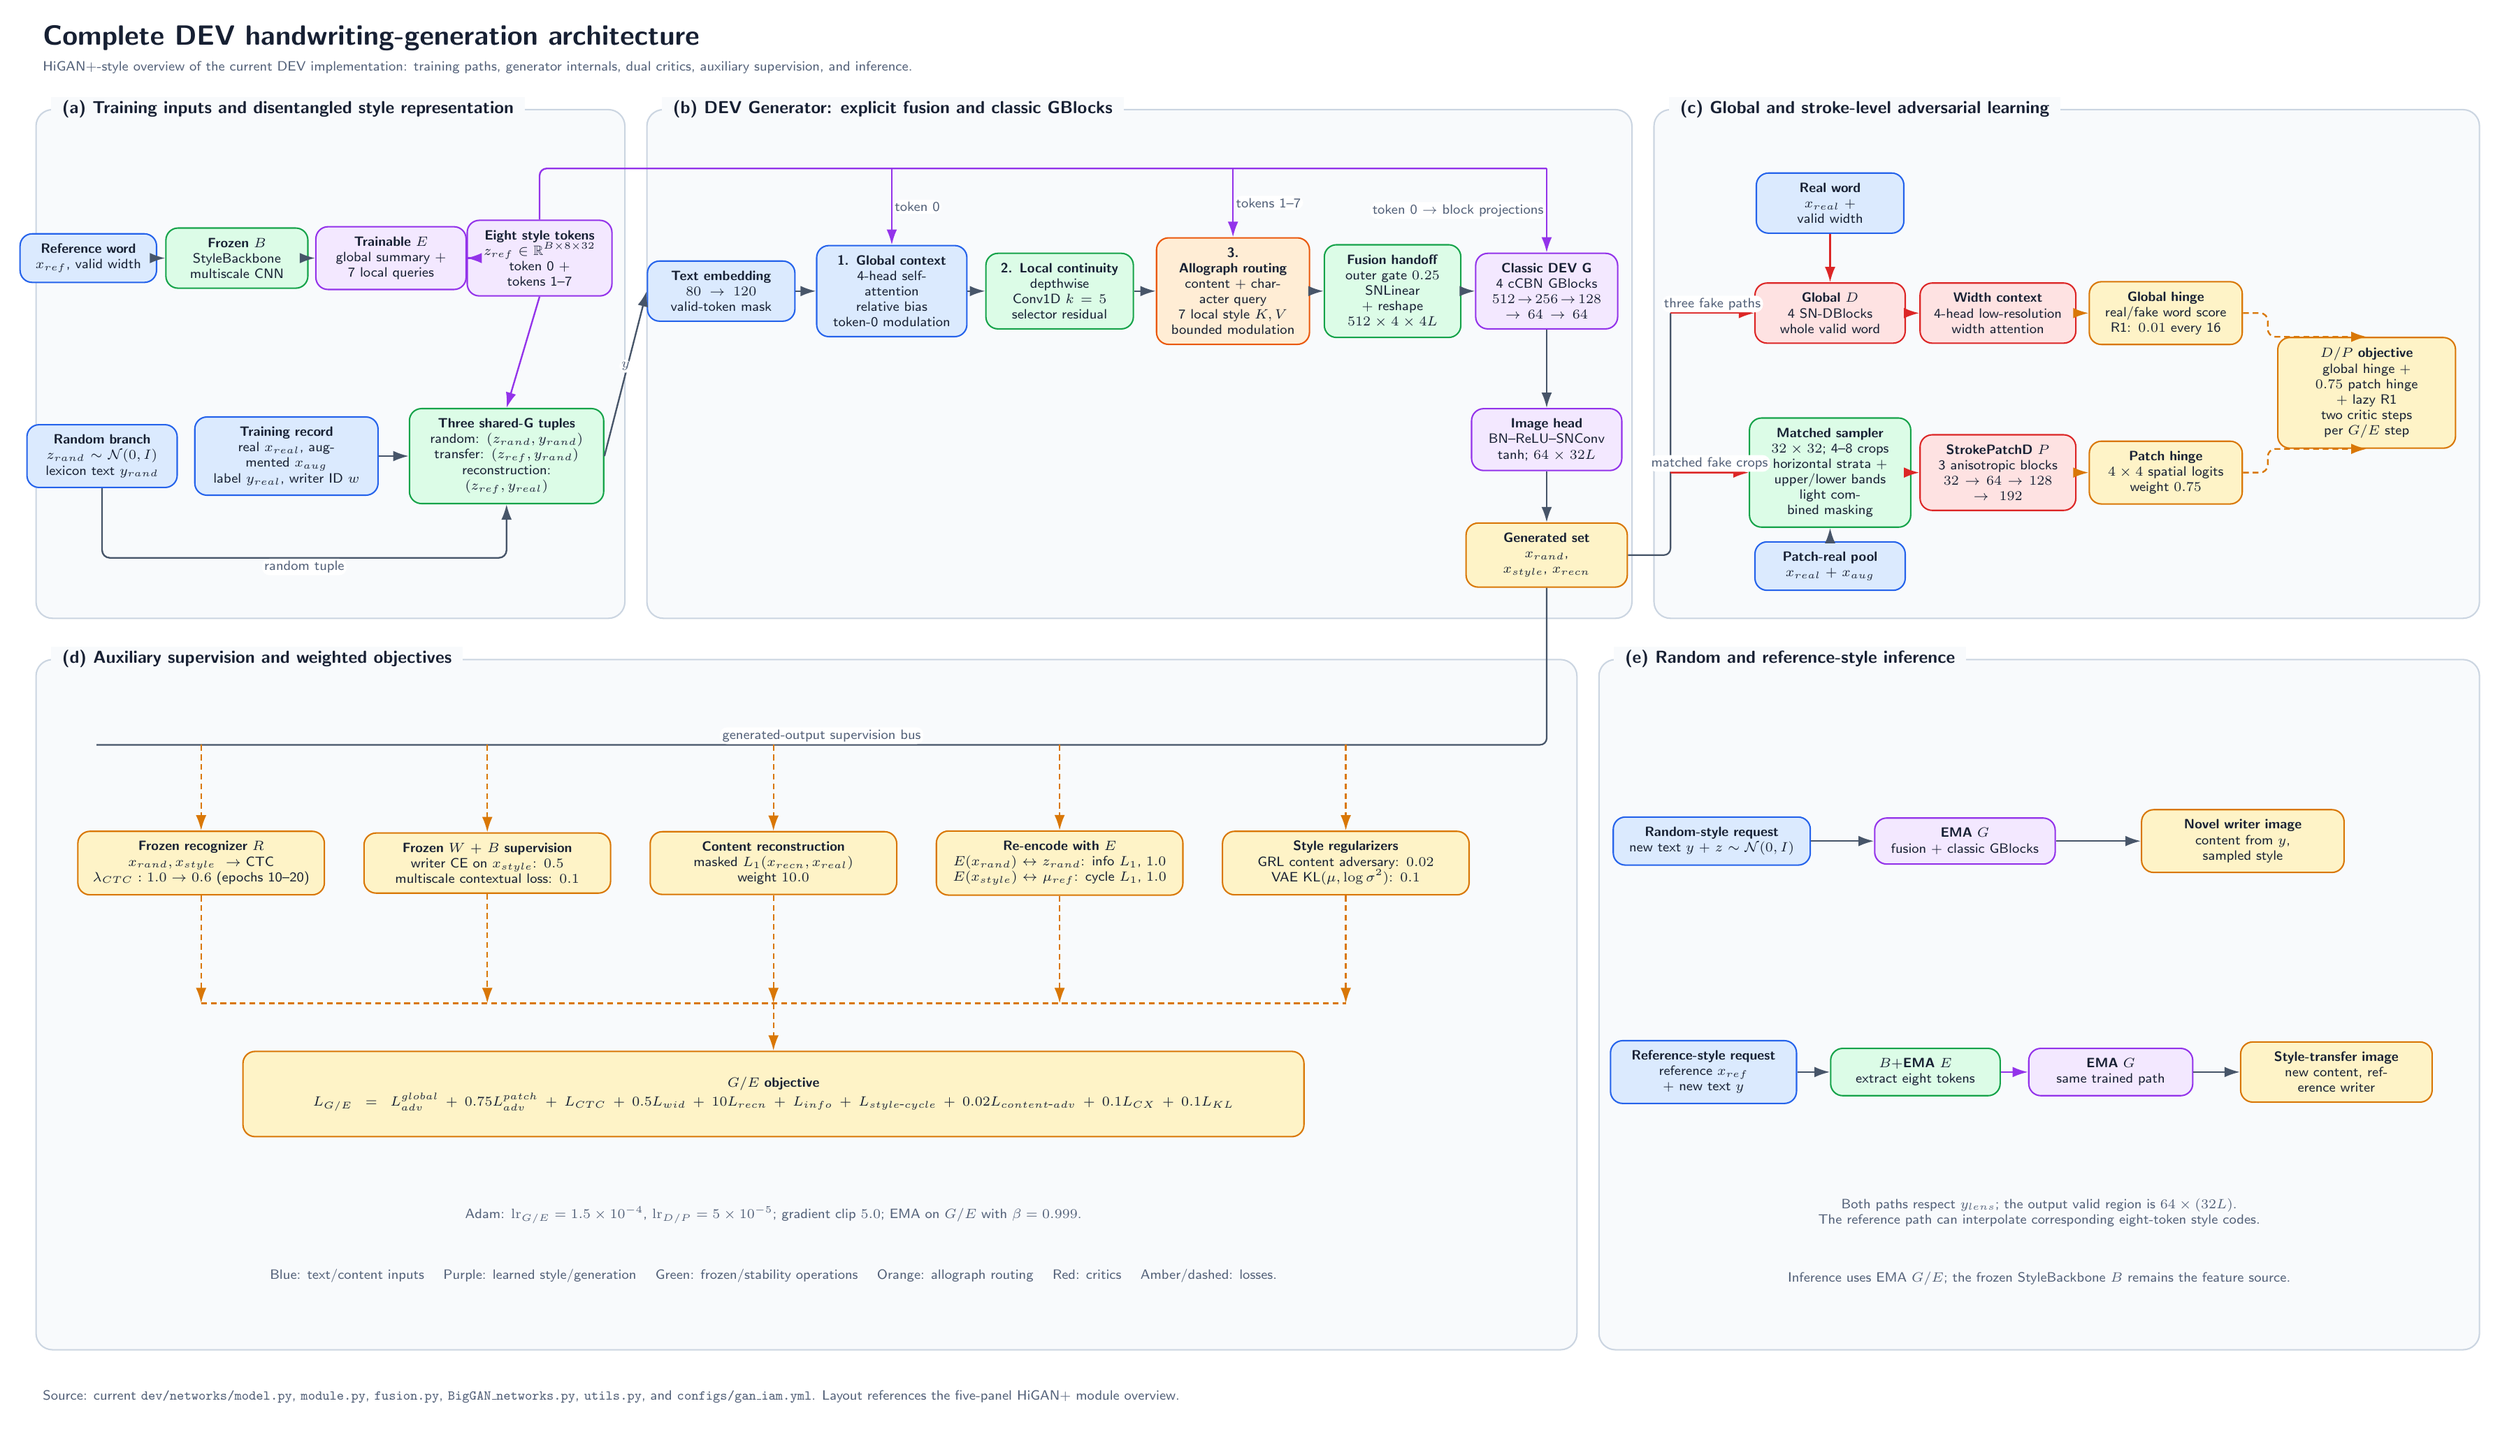
\begin{tikzpicture}[x=1cm,y=1cm]
  \node[font=\sffamily\bfseries\Large, text=DevInk, anchor=west]
    at (0,20.15) {Complete DEV handwriting-generation architecture};
  \node[devnote, anchor=west]
    at (0,19.62) {HiGAN+-style overview of the current DEV implementation: training paths, generator internals, dual critics, auxiliary supervision, and inference.};

  % Fixed panel bounds keep the five-part HiGAN+-inspired composition stable.
  \coordinate (aNW) at (0,18.85);
  \coordinate (aSE) at (10.70,9.60);
  \coordinate (bNW) at (11.10,18.85);
  \coordinate (bSE) at (29.00,9.60);
  \coordinate (cNW) at (29.40,18.85);
  \coordinate (cSE) at (44.40,9.60);
  \coordinate (dNW) at (0,8.85);
  \coordinate (dSE) at (28.00,-3.70);
  \coordinate (eNW) at (28.40,8.85);
  \coordinate (eSE) at (44.40,-3.70);

  % (a) Training inputs and style representation.
  \node[wholeinput, text width=2.0cm] (refimg) at (0.95,16.15)
    {\textbf{Reference word}\\$x_{ref}$, valid width};
  \node[wholestable, text width=2.1cm] (backbone) at (3.65,16.15)
    {\textbf{Frozen $B$}\\StyleBackbone\\multiscale CNN};
  \node[wholestyle, text width=2.25cm] (encoder) at (6.45,16.15)
    {\textbf{Trainable $E$}\\global summary +\\7 local queries};
  \node[wholestyle, text width=2.15cm] (tokens) at (9.15,16.15)
    {\textbf{Eight style tokens}\\$z_{ref}\in\mathbb{R}^{B\times8\times32}$\\token 0 + tokens 1--7};

  \draw[devflow] (refimg) -- (backbone);
  \draw[devflow] (backbone) -- (encoder);
  \draw[styleflow] (encoder) -- (tokens);

  \node[wholeinput, text width=2.25cm] (randompair) at (1.20,12.55)
    {\textbf{Random branch}\\$z_{rand}\sim\mathcal N(0,I)$\\lexicon text $y_{rand}$};
  \node[wholeinput, text width=2.85cm] (record) at (4.55,12.55)
    {\textbf{Training record}\\real $x_{real}$, augmented $x_{aug}$\\label $y_{real}$, writer ID $w$};
  \node[wholestable, text width=3.05cm] (batchpack) at (8.55,12.55)
    {\textbf{Three shared-G tuples}\\random: $(z_{rand},y_{rand})$\\transfer: $(z_{ref},y_{rand})$\\reconstruction: $(z_{ref},y_{real})$};

  \draw[devflow] (record) -- (batchpack);
  \draw[styleflow] (tokens.south) -- (batchpack.north);
  \coordinate (randomlaneL) at (1.20,10.70);
  \coordinate (randomlaneR) at (8.55,10.70);
  \draw[devflow] (randompair.south) -- (randomlaneL) --
    node[devlabel,below] {random tuple} (randomlaneR) -- (batchpack.south);

  % (b) Generator internals.
  \node[wholeinput, text width=2.2cm] (embed) at (12.45,15.55)
    {\textbf{Text embedding}\\$80\rightarrow120$\\valid-token mask};
  \node[wholeinput, text width=2.25cm] (context) at (15.55,15.55)
    {\textbf{1. Global context}\\4-head self-attention\\relative bias\\token-0 modulation};
  \node[wholestable, text width=2.2cm] (continuity) at (18.60,15.55)
    {\textbf{2. Local continuity}\\depthwise Conv1D $k=5$\\selector residual};
  \node[wholeallograph, text width=2.3cm] (allograph) at (21.75,15.55)
    {\textbf{3. \mbox{Allograph routing}}\\content + character query\\7 local style $K,V$\\bounded modulation};
  \node[wholestable, text width=2.0cm] (filter) at (24.65,15.55)
    {\textbf{Fusion handoff}\\outer gate $0.25$\\SNLinear + reshape\\$512\times4\times4L$};
  \node[wholestyle, text width=2.1cm] (gblocks) at (27.45,15.55)
    {\textbf{Classic DEV G}\\4 cCBN GBlocks\\$512\!\rightarrow\!256\!\rightarrow\!128$\\$\rightarrow64\rightarrow64$};
  \node[wholestyle, text width=2.25cm] (outhead) at (27.45,12.85)
    {\textbf{Image head}\\BN--ReLU--SNConv\\tanh; $64\times32L$};
  \node[wholeloss, text width=2.45cm] (generated) at (27.45,10.75)
    {\textbf{Generated set}\\$x_{rand}$, $x_{style}$, $x_{recn}$};

  \draw[devflow] (batchpack.east) -- node[devlabel,above] {$y$} (embed.west);
  \draw[devflow] (embed) -- (context);
  \draw[devflow] (context) -- (continuity);
  \draw[devflow] (continuity) -- (allograph);
  \draw[devflow] (allograph) -- (filter);
  \draw[devflow] (filter) -- (gblocks);
  \draw[devflow] (gblocks) -- (outhead);
  \draw[devflow] (outhead) -- (generated);

  % Explicit style-token bus: token 0 has two global jobs, local tokens have one.
  \coordinate (stylebusL) at (9.15,17.78);
  \coordinate (stylebusR) at (27.45,17.78);
  \draw[draw=DevStyleBorder,line width=0.85pt,rounded corners=1.3mm]
    (tokens.north) -- (stylebusL) -- (stylebusR);
  \draw[styleflow] (15.55,17.78) -- node[devlabel,right] {token 0} (context.north);
  \draw[styleflow] (21.75,17.78) -- node[devlabel,right] {tokens 1--7} (allograph.north);
  \draw[styleflow] (27.45,17.78) -- node[devlabel,left] {token 0 $\rightarrow$ block projections} (gblocks.north);

  % (c) Global and local adversarial supervision.
  \node[wholeinput, text width=2.2cm] (realglobal) at (32.60,17.15)
    {\textbf{Real word}\\$x_{real}$ + valid width};
  \node[wholecritic, text width=2.25cm] (globald) at (32.60,15.15)
    {\textbf{Global $D$}\\4 SN-DBlocks\\whole valid word};
  \node[wholecritic, text width=2.35cm] (widthmix) at (35.65,15.15)
    {\textbf{Width context}\\4-head low-resolution\\width attention};
  \node[wholeloss, text width=2.3cm] (globalhinge) at (38.70,15.15)
    {\textbf{Global hinge}\\real/fake word score\\R1: $0.01$ every 16};

  \node[wholeinput, text width=2.25cm] (realpatch) at (32.60,10.55)
    {\textbf{Patch-real pool}\\$x_{real}+x_{aug}$};
  \node[wholestable, text width=2.45cm] (patchsample) at (32.60,12.25)
    {\textbf{Matched sampler}\\$32\times32$; 4--8 crops\\horizontal strata + upper/lower bands\\light combined masking};
  \node[wholecritic, text width=2.35cm] (patchd) at (35.65,12.25)
    {\textbf{StrokePatchD $P$}\\3 anisotropic blocks\\$32\rightarrow64\rightarrow128$\\$\rightarrow192$};
  \node[wholeloss, text width=2.3cm] (patchhinge) at (38.70,12.25)
    {\textbf{Patch hinge}\\$4\times4$ spatial logits\\weight $0.75$};
  \node[wholeloss, text width=2.75cm] (dobjective) at (42.35,13.70)
    {\textbf{$D/P$ objective}\\global hinge + $0.75$ patch hinge\\+ lazy R1\\two critic steps per $G/E$ step};

  \draw[criticflow] (realglobal.south) -- (globald.north);
  \draw[criticflow] (globald) -- (widthmix);
  \draw[devlossflow] (widthmix) -- (globalhinge);
  \draw[devflow] (realpatch.north) -- (patchsample.south);
  \draw[criticflow] (patchsample) -- (patchd);
  \draw[devlossflow] (patchd) -- (patchhinge);
  \draw[devlossflow] (globalhinge.east) -- ++(0.45,0) |- (dobjective.north);
  \draw[devlossflow] (patchhinge.east) -- ++(0.45,0) |- (dobjective.south);

  % Generated-image bus enters both critics without crossing either branch.
  \coordinate (fakebus) at (29.70,10.75);
  \coordinate (fakebusTop) at (29.70,15.15);
  \coordinate (fakebusPatch) at (29.70,12.25);
  \draw[thinbus] (generated.east) -- (fakebus) -- (fakebusTop);
  \draw[criticflow] (fakebusTop) -- node[devlabel,above] {three fake paths} (globald.west);
  \draw[criticflow] (fakebusPatch) -- node[devlabel,above] {matched fake crops} (patchsample.west);

  % (d) Auxiliary supervision and weighted generator objective.
  \coordinate (genbusR) at (27.45,7.30);
  \coordinate (genbusL) at (1.10,7.30);
  \draw[thinbus] (generated.south) -- (genbusR) --
    node[devlabel,above] {generated-output supervision bus} (genbusL);

  \node[wholeloss, text width=4.0cm] (ctc) at (3.00,5.15)
    {\textbf{Frozen recognizer $R$}\\$x_{rand},x_{style}\rightarrow$ CTC\\$\lambda_{CTC}:1.0\rightarrow0.6$ (epochs 10--20)};
  \node[wholeloss, text width=4.0cm] (writerctx) at (8.20,5.15)
    {\textbf{Frozen $W+B$ supervision}\\writer CE on $x_{style}$: $0.5$\\multiscale contextual loss: $0.1$};
  \node[wholeloss, text width=4.0cm] (reconstruction) at (13.40,5.15)
    {\textbf{Content reconstruction}\\masked $L_1(x_{recn},x_{real})$\\weight $10.0$};
  \node[wholeloss, text width=4.0cm] (cycles) at (18.60,5.15)
    {\textbf{Re-encode with $E$}\\$E(x_{rand})\leftrightarrow z_{rand}$: info $L_1$, $1.0$\\$E(x_{style})\leftrightarrow\mu_{ref}$: cycle $L_1$, $1.0$};
  \node[wholeloss, text width=4.0cm] (regularizers) at (23.80,5.15)
    {\textbf{Style regularizers}\\GRL content adversary: $0.02$\\VAE KL$(\mu,\log\sigma^2)$: $0.1$};

  \foreach \x/\target in {3.00/ctc,8.20/writerctx,13.40/reconstruction,18.60/cycles,23.80/regularizers}
    \draw[devlossflow] (\x,7.30) -- (\target.north);

  \coordinate (losscollectL) at (3.00,2.60);
  \coordinate (losscollectR) at (23.80,2.60);
  \draw[lossbus] (losscollectL) -- (losscollectR);
  \foreach \target in {ctc,writerctx,reconstruction,cycles,regularizers}
    \draw[devlossflow] (\target.south) -- (\target.south |- losscollectL);

  \node[wholeloss, text width=18.8cm, minimum height=1.55cm] (gobjective) at (13.40,0.95)
    {\textbf{$G/E$ objective}\\
     $L_{G/E}=L_{adv}^{global}+0.75L_{adv}^{patch}+L_{CTC}+0.5L_{wid}+10L_{recn}+L_{info}+L_{style\mbox{-}cycle}+0.02L_{content\mbox{-}adv}+0.1L_{CX}+0.1L_{KL}$};
  \draw[devlossflow] (13.40,2.60) -- (gobjective.north);
  \node[devnote, align=center] at (13.40,-1.25)
    {Adam: $\mathrm{lr}_{G/E}=1.5\times10^{-4}$, $\mathrm{lr}_{D/P}=5\times10^{-5}$; gradient clip $5.0$; EMA on $G/E$ with $\beta=0.999$.};
  \node[devnote, align=center] at (13.40,-2.35)
    {Blue: text/content inputs \quad Purple: learned style/generation \quad Green: frozen/stability operations \quad Orange: allograph routing \quad Red: critics \quad Amber/dashed: losses.};

  % (e) Inference paths.
  \node[wholeinput, text width=3.1cm] (randomtest) at (30.45,5.55)
    {\textbf{Random-style request}\\new text $y$ + $z\sim\mathcal N(0,I)$};
  \node[wholestyle, text width=2.8cm] (emag1) at (35.05,5.55)
    {\textbf{EMA $G$}\\fusion + classic GBlocks};
  \node[wholeloss, text width=3.2cm] (randomout) at (40.10,5.55)
    {\textbf{Novel writer image}\\content from $y$, sampled style};
  \draw[devflow] (randomtest) -- (emag1);
  \draw[devflow] (emag1) -- (randomout);

  \node[wholeinput, text width=2.9cm] (reftest) at (30.30,1.35)
    {\textbf{Reference-style request}\\reference $x_{ref}$ + new text $y$};
  \node[wholestable, text width=2.6cm] (emaenc) at (34.15,1.35)
    {\textbf{$B+$EMA $E$}\\extract eight tokens};
  \node[wholestyle, text width=2.5cm] (emag2) at (37.70,1.35)
    {\textbf{EMA $G$}\\same trained path};
  \node[wholeloss, text width=3.0cm] (styleout) at (41.80,1.35)
    {\textbf{Style-transfer image}\\new content, reference writer};
  \draw[devflow] (reftest) -- (emaenc);
  \draw[styleflow] (emaenc) -- (emag2);
  \draw[devflow] (emag2) -- (styleout);

  \node[devnote, align=center] at (36.40,-1.20)
    {Both paths respect $y_{lens}$; the output valid region is $64\times(32L)$.\\The reference path can interpolate corresponding eight-token style codes.};
  \node[devnote, align=center] at (36.40,-2.40)
    {Inference uses EMA $G/E$; the frozen StyleBackbone $B$ remains the feature source.};

  % Panel backgrounds and labels are drawn last, behind all content and routes.
  \begin{scope}[on background layer]
    \node[devgroup, fit=(aNW)(aSE), inner sep=0pt] (panelA) {};
    \node[devgroup, fit=(bNW)(bSE), inner sep=0pt] (panelB) {};
    \node[devgroup, fit=(cNW)(cSE), inner sep=0pt] (panelC) {};
    \node[devgroup, fit=(dNW)(dSE), inner sep=0pt] (panelD) {};
    \node[devgroup, fit=(eNW)(eSE), inner sep=0pt] (panelE) {};
  \end{scope}
  \node[paneltitle, anchor=west] at ($(panelA.north west)+(0.28,0)$)
    {(a) Training inputs and disentangled style representation};
  \node[paneltitle, anchor=west] at ($(panelB.north west)+(0.28,0)$)
    {(b) DEV Generator: explicit fusion and classic GBlocks};
  \node[paneltitle, anchor=west] at ($(panelC.north west)+(0.28,0)$)
    {(c) Global and stroke-level adversarial learning};
  \node[paneltitle, anchor=west] at ($(panelD.north west)+(0.28,0)$)
    {(d) Auxiliary supervision and weighted objectives};
  \node[paneltitle, anchor=west] at ($(panelE.north west)+(0.28,0)$)
    {(e) Random and reference-style inference};

  \node[devnote, anchor=west] at (0,-4.55)
    {Source: current \texttt{dev/networks/model.py}, \texttt{module.py}, \texttt{fusion.py}, \texttt{BigGAN\_networks.py}, \texttt{utils.py}, and \texttt{configs/gan\_iam.yml}. Layout references the five-panel HiGAN+ module overview.};
\end{tikzpicture}
\end{document}
